% techinfo.tex
% $Header: techinfo.tex,v 0.1$

\section{Hardware}\label{sec:hardware}

Configurations will run on the cluster named "Athena". This is a IBM iDataPlex dx 360 m4 cluster. The idataplex cluster at CMCC is an Intel Xeon (Sandy Bridge E5-2670) system with the following characteristics:
\begin{itemize}
\item 8-core socket @ 2.6 GHz (with 3.0/3.3 turbo modes)
\begin{itemize}
\item 32KB 8-way L1 cache, instruction + data per core
\item 256kb L2 cache per core
\item 20 MB L3 cache (shared)
\item 20.8 GFlops peak performance per core
\item Support for 2 HyperThreading instances per core, 32 hyperthreads per node 
\end{itemize}
\item 2 sockets per node, 16 core per node
\item 4 memory controllers/socket
\item 51.2 GB/s memory bandwidth per socket
\item 64 GB memory/node (4GB/core), DDR3 1600MHz
\item 14x Infiniband FDR10 interconnect on PCIe3 (40 Gb/s = 5 GB/s unidirectional b/w)
\end{itemize}

For an extensive information about hardware specification and architecture you can see the "PELAGOS Activity Report"\cite{brunson_report} 

\section{Software}\label{sec:software}

Profiling in information science, refers to the ``process of construction and application of profiles generated by computerized data analysis''. Application of profiles will let us to measure the performance of applications. Profiling combined with rerunning previously completed tests and checking whether program behavior has changed (regression test) serve as a guidance to detection of newly introduced bugs. This early detection of errors is fundamental to assure the reliability of programs output, as a BFM climate predictions results. With the objective of automatize the profiling process of BFM, the tool {\it BFMtest} has been created.

\subsubsection{BFMtest}\label{subsubsec:soft_bfmtest}
{\it BFMtest} is the tool for testing configurations in BFM. This tool automatize the process of compiling, running and analyzing the different existing presets of BFM. Similar to the configuration tool for BFM (bfm\_configure), the configuration of a series of tests is based on presets and it is programmed using PERL\cite{perl.org} language. The analysis is carried out by other sub-tools (Valgrind\cite{valgrind} and nccmp\cite{nccmp}) and the outputs of these programs are inspected and summarized to show a complete report of tests.
\\\\
Similarly to {\it bfm\_configure}, {\it BFMtest} proceeding is divided in different phases. In total there are three phases:
\begin{itemize}
\item[{\bf Generation}:] Generate the test in the output directory. For that this phase will perform the generation, compilation and deployment steps of {\it bfm\_configure} with the default configuration modified by the particular options of the {\it BFMtest} preset.
\item[{\bf Run}:] Perform the execution of the test in the output directory. This phase includes waiting for the process to finish the run (also if is a batch job)  
\item[{\bf Analysis}:] Build the summary of the generation and run. It will collect if the previous phases were successful, show run-time and status of the optional diagnostics (Valgrind and comparison)  
\end{itemize}\bigskip

The execution of one preset will entails the execution of one or several tests ({\it bfm\_configure} presets). The cycle of execution is, for each test performs the selected phases (Generations, Run and Analysis) consecutively and continue to next one. Then each test is treated independently, even if they are in the same {\it BFMtest} preset. See image \ref{fig:bfmtest}. The command to run the tool with an specific preset is:
\begin{lstlisting}[language=bash]
bfm_configure.sh -p PRESET_NAME
\end{lstlisting}
You can also use the verbose mode for getting more information:
\begin{lstlisting}[language=bash]
bfm_configure.sh -vp PRESET_NAME
\end{lstlisting}
\clearpage
The following table summarize available options. For a up-to-date options table check the "EXAMPLE" file in the configuration directories.
\begin{itemize}
\item[{\bf NAME}:] Name of the test (mandatory)
\item[{\bf ACTIVE}:] Specify execution stage to perform. Valid values are (you can combine them):
  \begin{itemize}
  \item[{\bf Y}:] all execution stages: generation, running and analysis (default)
  \item[{\bf N}:] no execution. Test will not be generated, run or analyzed. 
  \item[{\bf G}:] only generation
  \item[{\bf R}:] only running
  \item[{\bf A}:] only analysis
  \end{itemize}
\item[{\bf PRESET}:] Name of the preset for using as parameter in {\it bfm\_configure} (see {\it bfm\_configure} option '-p')
\item[{\bf COPY}:] Copy other generated test
  \begin{itemize}
  \item In generation time, The test will not be generated, only copied and deployed ({\it bfm\_configure} option '-d')
  \item Source test must exists in tmp directory (use ACTIVE=G to only execute generation of source test) 
  \end{itemize}
\item[{\bf RUN}:] Mode to run the experiment. Valid values are:
  \begin{itemize}
  \item[{\bf sh}:] default, for running in a unix shell
  \item[{\bf bsub}:] for running in batch mode
  \end{itemize}
\item[{\bf RUNEXE}:] Specify prototype for generating the experiment running script (see {\it bfm\_configure} option '-R')
\item[{\bf PROC}:] Number of processors to use in compilation and running (see {\it bfm\_configure} option '-r')
\item[{\bf ARCH}:] Specify compilation Architecture file (see {\it bfm\_configure} option '-a')
\item[{\bf QUEUE}:] Specify queue in job mode (see {\it bfm\_configure} option '-q')
\item[{\bf PAREXE}:] Command to execute in parallel. Ex: openmpirun (see {\it bfm\_configure} option '-e')
  \begin{itemize}
  \item You can use \$PROC inside this command
  \end{itemize}
\item[{\bf PRECMD}:] Commands to execute prior compiling and prior running
\item[{\bf PRERUN}:] Commands to execute prior running 
\item[{\bf FORCING}:] Forcing files to link in the run directory (see {\it bfm\_configure} option '-i')
\item[{\bf VALGRIND}:] Valgrind command and options for analysis
\item[{\bf COMPARE}:] Directory with test output to compare results
  \begin{itemize}
  \item Run command "nccmp -V" first to check if nccmp command works
  \end{itemize}
\item[{\bf COMPTHR}:] Compare threshold for nccmp command (default 1e-3)
\end{itemize}\bigskip

All the options follow these rules for specification of values: 
\begin{itemize}
\item Options are separated by lines, and values by coma ','
\item Write an option in multiple lines using backslash '\textbackslash' at the end of the line
\item Use two single quotes '' to specify empty values.
\end{itemize}\bigskip

\begin{sidewaysfigure*}
  \centering
  \includegraphics[angle=90]{img/bfmtest.ps}
  \caption{BFMtest flow diagram}
  \label{fig:bfmtest}
\end{sidewaysfigure*}
\clearpage

\subsection{Tools}\label{subsec:soft_tools}
\subsubsection{NCCMP}\label{subsubsec:tools_nccmp}

Nccmp compares two NetCDF files bitwise or with a user defined tolerance (absolute or relative percentage). Comparisons are done in local memory without requiring temporary files. This tool is very useful for running regression test of scientific models.

As an example you can execute the command:
\begin{lstlisting}[language=bash]
nccmp -dgmf NETCDF_FILE1 NETCDF_FILE2
\end{lstlisting}
This command will compare the data (-d), global attributes (-g), metadata (-m) and will execute the comparison until the end (-f).

To download and learn how to use it go the tool online web page\cite{nccmp}).

\subsubsection{Valgrind}\label{subsubsec:tools_valgrind}

Valgrind is an strumentation frameworks for building analysis tools. Valgrind distribution contains useful quality tools. The tools used in this report are these:
\begin{itemize}
\item{{\bf Callgrind}\cite{val_callgrind}} is a profiling tool that records the call history among functions in a program's run as a call-graph. By default, the collected data consists of the number of instructions executed, their relationship to source lines, the caller/callee relationship between functions, and the numbers of such calls. Optionally, cache simulation and/or branch prediction (similar to Cachegrind) can produce further information about the runtime behavior of an application.
\item{{\bf Massif}\cite{val_massif}} is a heap profiler. It measures how much heap memory your program uses. This includes both the useful space, and the extra bytes allocated for book-keeping and alignment purposes.
\end{itemize}

For more information of these tools, go to the online web page \cite{valgrind}.
\\\\
Other useful tools related with Valgrind but developed independiently are:
\begin{itemize}
\item{{\bf KCachegrind}\cite{kcachegrind}} Callgrind output visualizer.
\item{{\bf Massif-Visualizer}\cite{massif-visualizer}} Massif output visualizer.
\end{itemize}
